\documentclass[8pt]{beamer}

% Beamer style
%\usetheme[secheader]{Madrid}
% \usetheme{CambridgeUS}
\useoutertheme{infolines}
\usecolortheme[rgb={0.65,0.15,0.25}]{structure}
% \usefonttheme[onlymath]{serif}
\beamertemplatenavigationsymbolsempty
%\AtBeginSubsection

% Packages
%\usepackage[french]{babel}
\usepackage[latin1]{inputenc}
\usepackage{color}
% \usepackage[dvipsnames]{xcolor}
\usepackage{xspace}
\usepackage{dsfont, stmaryrd}
\usepackage{amsmath, amsfonts, amssymb, stmaryrd, mathabx}
\usepackage{epsfig}
\usepackage{tikz}
\usepackage{url}
% \usepackage{ulem}
\usepackage{/home/robin/LATEX/Biblio/astats}
%\usepackage[all]{xy}
\usepackage{graphicx}

% Maths
% \newtheorem{theorem}{Theorem}
% \newtheorem{definition}{Definition}
\newtheorem{proposition}{Proposition}
% \newtheorem{assumption}{Assumption}
% \newtheorem{algorithm}{Algorithm}
% \newtheorem{lemma}{Lemma}
% \newtheorem{remark}{Remark}
% \newtheorem{exercise}{Exercise}
% \newcommand{\propname}{Prop.}
% \newcommand{\proof}{\noindent{\sl Proof:}\quad}
% \newcommand{\eproof}{$\blacksquare$}

% \setcounter{secnumdepth}{3}
% \setcounter{tocdepth}{3}
\newcommand{\pref}[1]{\ref{#1} p.\pageref{#1}}
\newcommand{\qref}[1]{\eqref{#1} p.\pageref{#1}}

% Colors : http://latexcolor.com/
\definecolor{darkred}{rgb}{0.65,0.15,0.25}
\definecolor{darkgreen}{rgb}{0,0.4,0}
\definecolor{darkred}{rgb}{0.65,0.15,0.25}
\definecolor{amethyst}{rgb}{0.6, 0.4, 0.8}
\definecolor{asparagus}{rgb}{0.53, 0.66, 0.42}
\definecolor{applegreen}{rgb}{0.55, 0.71, 0.0}
\definecolor{awesome}{rgb}{1.0, 0.13, 0.32}
\definecolor{blue-green}{rgb}{0.0, 0.87, 0.87}
\definecolor{red-ggplot}{rgb}{0.52, 0.25, 0.23}
\definecolor{green-ggplot}{rgb}{0.42, 0.58, 0.00}
\definecolor{purple-ggplot}{rgb}{0.34, 0.21, 0.44}
\definecolor{blue-ggplot}{rgb}{0.00, 0.49, 0.51}

% Commands
\newcommand{\backupbegin}{
   \newcounter{finalframe}
   \setcounter{finalframe}{\value{framenumber}}
}
\newcommand{\backupend}{
   \setcounter{framenumber}{\value{finalframe}}
}
\newcommand{\emphase}[1]{\textcolor{darkred}{#1}}
\newcommand{\comment}[1]{\textcolor{gray}{#1}}
\newcommand{\paragraph}[1]{\textcolor{darkred}{#1}}
\newcommand{\refer}[1]{{\small{\textcolor{gray}{{\cite{#1}}}}}}
\newcommand{\Refer}[1]{{\small{\textcolor{gray}{{[#1]}}}}}
\newcommand{\goto}[1]{{\small{\textcolor{blue}{[\#\ref{#1}]}}}}
\renewcommand{\newblock}{}

\newcommand{\tabequation}[1]{{\medskip \centerline{#1} \medskip}}
% \renewcommand{\binom}[2]{{\left(\begin{array}{c} #1 \\ #2 \end{array}\right)}}

% Variables 
\newcommand{\Abf}{{\bf A}}
\newcommand{\Beta}{\text{B}}
\newcommand{\Bcal}{\mathcal{B}}
\newcommand{\Bias}{\xspace\mathbb B}
\newcommand{\Cor}{{\mathbb C}\text{or}}
\newcommand{\Cov}{{\mathbb C}\text{ov}}
\newcommand{\cl}{\text{\it c}\ell}
\newcommand{\Ccal}{\mathcal{C}}
\newcommand{\cst}{\text{cst}}
\newcommand{\Dcal}{\mathcal{D}}
\newcommand{\Ecal}{\mathcal{E}}
\newcommand{\Esp}{\xspace\mathbb E}
\newcommand{\Espt}{\widetilde{\Esp}}
\newcommand{\Covt}{\widetilde{\Cov}}
\newcommand{\Ibb}{\mathbb I}
\newcommand{\Fcal}{\mathcal{F}}
\newcommand{\Gcal}{\mathcal{G}}
\newcommand{\Gam}{\mathcal{G}\text{am}}
\newcommand{\Hcal}{\mathcal{H}}
\newcommand{\Jcal}{\mathcal{J}}
\newcommand{\Lcal}{\mathcal{L}}
\newcommand{\Mt}{\widetilde{M}}
\newcommand{\mt}{\widetilde{m}}
\newcommand{\Nbb}{\mathbb{N}}
\newcommand{\Mcal}{\mathcal{M}}
\newcommand{\Ncal}{\mathcal{N}}
\newcommand{\Ocal}{\mathcal{O}}
\newcommand{\pt}{\widetilde{p}}
\newcommand{\Pt}{\widetilde{P}}
\newcommand{\Pbb}{\mathbb{P}}
\newcommand{\Pcal}{\mathcal{P}}
\newcommand{\Qcal}{\mathcal{Q}}
\newcommand{\qt}{\widetilde{q}}
\newcommand{\Rbb}{\mathbb{R}}
\newcommand{\Sbb}{\mathbb{S}}
\newcommand{\Scal}{\mathcal{S}}
\newcommand{\st}{\widetilde{s}}
\newcommand{\St}{\widetilde{S}}
\newcommand{\Tcal}{\mathcal{T}}
\newcommand{\todo}{\textcolor{red}{TO DO}}
\newcommand{\Ucal}{\mathcal{U}}
\newcommand{\Un}{\math{1}}
\newcommand{\Vcal}{\mathcal{V}}
\newcommand{\Var}{\mathbb V}
\newcommand{\Vart}{\widetilde{\Var}}
\newcommand{\Zcal}{\mathcal{Z}}

% Symboles & notations
\newcommand\independent{\protect\mathpalette{\protect\independenT}{\perp}}\def\independenT#1#2{\mathrel{\rlap{$#1#2$}\mkern2mu{#1#2}}} 
\renewcommand{\d}{\text{\xspace d}}
\newcommand{\gv}{\mid}
\newcommand{\ggv}{\, \| \, }
% \newcommand{\diag}{\text{diag}}
\newcommand{\card}[1]{\text{card}\left(#1\right)}
\newcommand{\trace}[1]{\text{tr}\left(#1\right)}
\newcommand{\matr}[1]{\boldsymbol{#1}}
\newcommand{\matrbf}[1]{\mathbf{#1}}
\newcommand{\vect}[1]{\matr{#1}} %% un peu inutile
\newcommand{\vectbf}[1]{\matrbf{#1}} %% un peu inutile
\newcommand{\trans}{\intercal}
\newcommand{\transpose}[1]{\matr{#1}^\trans}
\newcommand{\crossprod}[2]{\transpose{#1} \matr{#2}}
\newcommand{\tcrossprod}[2]{\matr{#1} \transpose{#2}}
\newcommand{\matprod}[2]{\matr{#1} \matr{#2}}
\DeclareMathOperator*{\argmin}{arg\,min}
\DeclareMathOperator*{\argmax}{arg\,max}
\DeclareMathOperator{\sign}{sign}
\DeclareMathOperator{\tr}{tr}
\newcommand{\ra}{\emphase{$\rightarrow$} \xspace}

% Hadamard, Kronecker and vec operators
\DeclareMathOperator{\Diag}{Diag} % matrix diagonal
\DeclareMathOperator{\diag}{diag} % vector diagonal
\DeclareMathOperator{\mtov}{vec} % matrix to vector
\newcommand{\kro}{\otimes} % Kronecker product
\newcommand{\had}{\odot}   % Hadamard product

% TikZ
\newcommand{\nodesize}{2em}
\newcommand{\edgeunit}{2.5*\nodesize}
\newcommand{\edgewidth}{1pt}
\tikzstyle{node}=[draw, circle, fill=black, minimum width=.75\nodesize, inner sep=0]
\tikzstyle{square}=[rectangle, draw]
\tikzstyle{param}=[draw, rectangle, fill=gray!50, minimum width=\nodesize, minimum height=\nodesize, inner sep=0]
\tikzstyle{hidden}=[draw, circle, fill=gray!50, minimum width=\nodesize, inner sep=0]
\tikzstyle{hiddenred}=[draw, circle, color=red, fill=gray!50, minimum width=\nodesize, inner sep=0]
\tikzstyle{observed}=[draw, circle, minimum width=\nodesize, inner sep=0]
\tikzstyle{observedred}=[draw, circle, minimum width=\nodesize, color=red, inner sep=0]
\tikzstyle{eliminated}=[draw, circle, minimum width=\nodesize, color=gray!50, inner sep=0]
\tikzstyle{empty}=[draw, circle, minimum width=\nodesize, color=white, inner sep=0]
\tikzstyle{blank}=[color=white]
\tikzstyle{nocircle}=[minimum width=\nodesize, inner sep=0]

\tikzstyle{edge}=[-, line width=\edgewidth]
\tikzstyle{edgebendleft}=[-, >=latex, line width=\edgewidth, bend left]
\tikzstyle{edgebendright}=[-, >=latex, line width=\edgewidth, bend right]
\tikzstyle{lightedge}=[-, line width=\edgewidth, color=gray!50]
\tikzstyle{lightedgebendleft}=[-, >=latex, line width=\edgewidth, bend left, color=gray!50]
\tikzstyle{lightedgebendright}=[-, >=latex, line width=\edgewidth, bend right, color=gray!50]
\tikzstyle{edgered}=[-, line width=\edgewidth, color=red]
\tikzstyle{edgebendleftred}=[-, >=latex, line width=\edgewidth, bend left, color=red]
\tikzstyle{edgebendrightred}=[-, >=latex, line width=\edgewidth, bend right, color=red]

\tikzstyle{arrow}=[->, >=latex, line width=\edgewidth]
\tikzstyle{arrowbendleft}=[->, >=latex, line width=\edgewidth, bend left]
\tikzstyle{arrowbendright}=[->, >=latex, line width=\edgewidth, bend right]
\tikzstyle{arrowred}=[->, >=latex, line width=\edgewidth, color=red]
\tikzstyle{arrowbendleftred}=[->, >=latex, line width=\edgewidth, bend left, color=red]
\tikzstyle{arrowbendrightred}=[->, >=latex, line width=\edgewidth, bend right, color=red]
\tikzstyle{arrowblue}=[->, >=latex, line width=\edgewidth, color=blue]
\tikzstyle{dashedarrow}=[->, >=latex, dashed, line width=\edgewidth]
\tikzstyle{dashededge}=[-, >=latex, dashed, line width=\edgewidth]
\tikzstyle{dashededgebendleft}=[-, >=latex, dashed, line width=\edgewidth, bend left]
\tikzstyle{lightarrow}=[->, >=latex, line width=\edgewidth, color=gray!50]

\newcommand{\bEDD}{BEDD\xspace}
\newcommand{\Fbar}{\overline{F}}
\newcommand{\phibar}{\overline{\phi}}

% Directory
\newcommand{\fignet}{/home/robin/RECHERCHE/RESEAUX/EXPOSES/FIGURES}

%====================================================================
%====================================================================

%====================================================================
%====================================================================
\begin{document}
%====================================================================
%====================================================================

%====================================================================
\title[Bipartite motifs]{Motif-based analysis of bipartite networks \\}

\author[S. Robin]{S. Robin \\ \medskip
joint work with S. Ouadah, P. Latouche \refer{OLR21}\\ ~}

\institute[]{INRA / AgroParisTech / univ. Paris-Saclay / Museum National d'Histoire Naturelle \\~ \\~}

\date[Paris, Apr.'21]{LPSM, Paris, Apr. 2021}

%====================================================================
%====================================================================
\maketitle
%====================================================================
\frame{\frametitle{Outline} \tableofcontents}
%====================================================================
%====================================================================
\section{Bipartite networks and motifs}
\frame{\frametitle{Outline} \tableofcontents[currentsection]}
%====================================================================
\frame{\frametitle{Bipartite network} 

  \hspace{-.04\textwidth}
  \begin{tabular}{cc}
    \begin{tabular}{p{.53\textwidth}}
      \paragraph{Bipartite graph.} Graph connecting to distinct types of nodes: 
      $$
      G = (E^{\circ}, E^{\square}, V)
      $$ 
      \begin{itemize}
      \item $E^{\circ} = $ 'top' nodes ($1 \leq i \leq m$) \\~ 
      \item $E^{\square} = $ 'bottom' nodes ($1 \leq j \leq n$) \\~ 
      \item $V \subset E^{\circ} \times E^{\square} =$ set of edges \\~ 
      \end{itemize}
      Equivalent to a $m \times n$ adjacency matrix $G$.
    \end{tabular}
    & 
    \hspace{-.05\textwidth} 
    \begin{tabular}{c} 
      Bipartite graph $G$ \\
      \includegraphics[width=.4\textwidth, trim=0 50 0 50]{\fignet/Zackenberg-1996_12-red-net} \\
      \includegraphics[width=.4\textwidth, angle=90, trim=0 50 0 50, clip]{\fignet/Zackenberg-1996_12-red-adj}
    \end{tabular}
  \end{tabular}

}

%====================================================================
\frame{\frametitle{Bipartite motif} 

  \hspace{-.04\textwidth}
  \begin{tabular}{cc}
    \begin{tabular}{p{.7\textwidth}}
      \paragraph{Bipartite motif.} Sub-graph ($p \ll m$, $q \ll n$) of a bipartite graph
      $$
      s = (\{1, \dots p\}, \{1, \dots q\}, A)
      $$
      \bigskip
      $$
      \text{Motif adjacency matrix (right):} \qquad A = \left( \begin{array}{cc} 0 & 1 \\ 0 & 1 \\ 1 & 1 \end{array} \right)
      $$
    \end{tabular}
    & 
    \hspace{-.05\textwidth} 
    \begin{tabular}{c} 
      Bipartite motif $s$ \\
      \includegraphics[width=.2\textwidth]{\fignet/FigMotifsBEDD-motif9-automorphism1}
    \end{tabular}
  \end{tabular}

  \bigskip \bigskip \bigskip 
  \paragraph{Motif count.}
  $$
  N_s = N_s(G) = \text{number of occurrences of the motif $s$ in the graph $G$}
  $$
}

%====================================================================
\frame{\frametitle{Motivation (1/2)} 

  \hspace{-.025\textwidth}
  \begin{tabular}{cc}
    \begin{tabular}{p{.45\textwidth}}
      \paragraph{Simmons \& al, 2019.} \\ ~
      \begin{itemize}
      \item Motifs in bipartite ecological networks: uncovering indirect interactions \\
      {\sl Oikos} \refer{SCB19} \\ ~
      \item {\tt bmotif} : A package for motif analyses of bipartite networks \\
      {\sl Methods in Ecology and Evolution} \refer{SSS19}
      \end{itemize}
    \end{tabular}
    & 
%     \hspace{-.05\textwidth}
    \begin{tabular}{p{.5\textwidth}}
      \includegraphics[width=.45\textwidth]{\fignet/SCB19-Oikos-Fig3-6motifs}
    \end{tabular}
  \end{tabular}

}

%====================================================================
\frame{\frametitle{Motivation (2/2)} 

  \paragraph{Bipartite ecological networks.}
  \begin{itemize}
  \item Plant-pollinator: $\circ =$ plants, $\square =$ insects (mutualistic)
  \item Host-parasite: $\circ =$ plants, $\square =$ herbivors (antagonistic)
  \end{itemize}
      
  \bigskip \bigskip \pause
  \paragraph{Motif counts} provide a generic 'meso-scale' description of a network \refer{SCB19}
  \begin{itemize}
  \item motifs = 'building-blocks'
  \item between local (node degree) and global ('metrics')
  \end{itemize}

  \bigskip \bigskip \pause
  \paragraph{Applications.}
  \begin{itemize}
  \item Describe networks 
  \item Compare a network to a null model 
  \item Compare networks (even when the nodes = species are different)
  \item \textcolor{gray}{Characterize species according their 'role' in various networks}
  \end{itemize} 

}

%====================================================================
\frame{\frametitle{Counting bipartite motifs} 

  \bigskip
  \paragraph{General motif.} 
  \begin{itemize}
   \item Counting is computationally demanding (\url{bmotif} package \refer{SSS19}: up to 6 nodes) \\ ~
   \item Need to account for automorphisms = non-redundant permutations of the motif's adjacency matrix:
   $$
   s = \includegraphics[width=.05\textwidth, trim=100 200 100 0]{\fignet/FigMotifsBEDD-motif9-automorphism1}: \qquad
   \left\{
   \includegraphics[width=.05\textwidth, trim=100 200 100 0]{\fignet/FigMotifsBEDD-motif9-automorphism1} \quad  
   \includegraphics[width=.05\textwidth, trim=100 200 100 0]{\fignet/FigMotifsBEDD-motif9-automorphism2} \quad 
   \includegraphics[width=.05\textwidth, trim=100 200 100 0]{\fignet/FigMotifsBEDD-motif9-automorphism3} \quad 
   \includegraphics[width=.05\textwidth, trim=100 200 100 0]{\fignet/FigMotifsBEDD-motif9-automorphism4} \quad 
   \includegraphics[width=.05\textwidth, trim=100 200 100 0]{\fignet/FigMotifsBEDD-motif9-automorphism5} \quad 
   \includegraphics[width=.05\textwidth, trim=100 200 100 0]{\fignet/FigMotifsBEDD-motif9-automorphism6}
   \right\} \quad
   \Rightarrow \quad \emphase{r_s = 6} \leq (p_s!) (q_s!)
   $$
  \end{itemize}
  
  \bigskip \bigskip \pause
  \paragraph{Star motif:} one node connected to $d$ nodes:
  top star = \includegraphics[width=.05\textwidth, trim=100 200 100 0]{\fignet/FigMotifsBEDD-motif7-automorphism1}, \quad
  bottom star = \includegraphics[width=.05\textwidth, trim=100 200 100 0]{\fignet/FigMotifsBEDD-motif8-automorphism1} 
        
  \bigskip \bigskip
  Easy to count: $r = 1$ and, denoting $G_{i+} = \sum_j G_{ij}$ the degree of the $i$th top node,
  $$
  N(\text{top star with degree $d$}) = \sum_{i = 1}^n \binom{G_{i+}}{d}
  $$
  
}

%====================================================================
\frame{\frametitle{Motif count} 

  To count the occurrences of motif $s$ in the graph $G$, we need to
  \begin{enumerate}
  \item visit each possible 'position' $\alpha \in \Pcal_s$, where
  $$
  \Pcal_s = 
  \{\text{$p_s$ top nodes among $m$}\} \times
  \{\text{$q_s$ top nodes among $n$}\} \times
  \{\text{$r_s$ automorphisms}\}
  $$
  so the total number of positions is 
  $$
  c_s := |\Pcal_s| = \binom{m}{p_s} \; \binom{n}{q_s} \; r_s
  $$ \pause
  \item for each position $\alpha$, check (for each permutation of $A$) if the motif matches
  $$
  Y_s(\alpha) 
  = \prod_{u = 1}^{p_s} \prod_{v = 1}^{q_s} G_{i_u, j_v}^{A_{u, v}}
  \comment{\neq \prod_{u = 1}^{p_s} \prod_{v = 1}^{q_s} G_{i_u, j_v}^{A_{u, v}} (1 - G_{i_u, j_v})^{1 - A_{u, v}}}
  $$
  (induced motif).
  \end{enumerate}
  
  \bigskip \pause
  \paragraph{Motif count.}
  $$
  N_s = \sum_{\alpha \in \Pcal_s} Y_s(\alpha)
  $$
  Motif frequency: $F_s := N_s / c_s$.
  
}

%====================================================================
\section{Bipartite expected degree distribution model}
\frame{\frametitle{Outline} \tableofcontents[currentsection]}
%====================================================================
\frame{\frametitle{A null model} 

  \bigskip
  \paragraph{\bEDD model.} A row-column exhangeable model: \\ ~
  \begin{itemize}
   \item $\{U_i\}_{1 \leq i \leq m} \text{ iid}: U_i \sim \Ucal_{[0, 1]}$, 
   \qquad $\{V_j\}_{1 \leq j \leq n} \text{ iid}: V_j \sim \Ucal_{[0, 1]}$, \\ ~
   \item $\{G_{ij}\}_{1 \leq i, \leq m, 1 \leq j \leq n} \text{ independent } \mid \{U_i\}, \{V_j\}:$
   $$
   \Pr\{G_{ij} = 1 \mid U_i, V_j\} = \rho \; g(U_i) \; h(V_j).
   $$
  \end{itemize}
  
  \bigskip 
  where:
  \begin{itemize}
  \item $\rho =$ network density, \\ ~
  \item $g =$ degree imbalance among top nodes ($g \geq 0$, $\int g(u) \d u = 1$)  \comment{(specialist vs generalist)}, \\ ~
  \item $h =$ degree imbalance among bottom nodes ($h \geq 0$, $\int h(v) \d v = 1$).
  \end{itemize}

  \bigskip \bigskip \pause
  \paragraph{Related models.} \bEDD model =
  \begin{itemize}
   \item bipartite exchangeable version of the (expected) degree sequence model \refer{MoR95,ChL02}
   \item bipartite product-form $W$-graph \refer{LoS06}: $w(u, v) = \rho g(u) h(v)$
  \end{itemize}

}

%==================================================================
\frame{\frametitle{\bEDD model}

  \begin{tabular}{rccc}
    & & $h =$ & $h =$ \\
%     \multicolumn{2}{c}{
%       $\begin{array}{rl}
%         \Pbb\{i \sim j \mid U_i, V_j\} & = \rho \; g(U_i) \; h(V_j) \\ \\
%         \Esp (D_i \mid U_i) & = n \; \rho \; g(U_i) \\ \\
%         \Esp (D_j \mid V_j) & = m \; \rho \; g(V_i) 
%       \end{array}$
%     } 
    \multicolumn{2}{l}{
      \begin{tabular}{rcl}
        top & = & rows \\
        ~ \\ 
        bottom & = & columns \\
      \end{tabular}
    } 
    &
    \begin{tabular}{c} 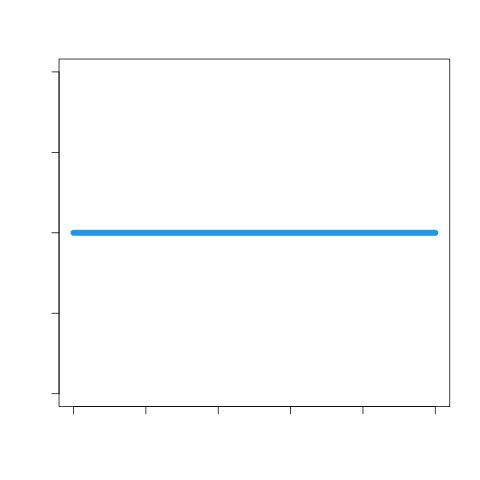
\includegraphics[width=.18\textwidth]{\fignet/FigMotifsBEDD-dist-h10} \end{tabular} &
    \begin{tabular}{c} 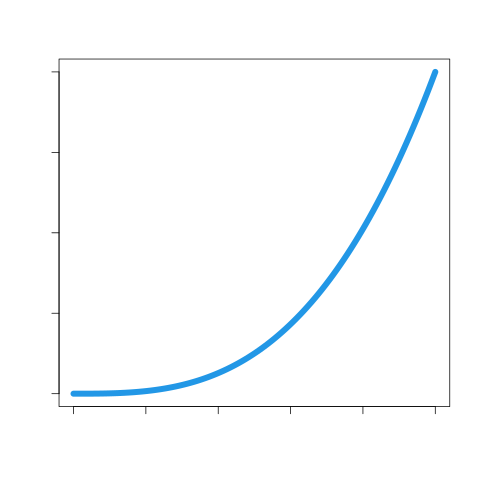
\includegraphics[width=.18\textwidth]{\fignet/FigMotifsBEDD-dist-h40} \end{tabular} \\
    \begin{tabular}{r} $g =$ \end{tabular} &
    \begin{tabular}{c} 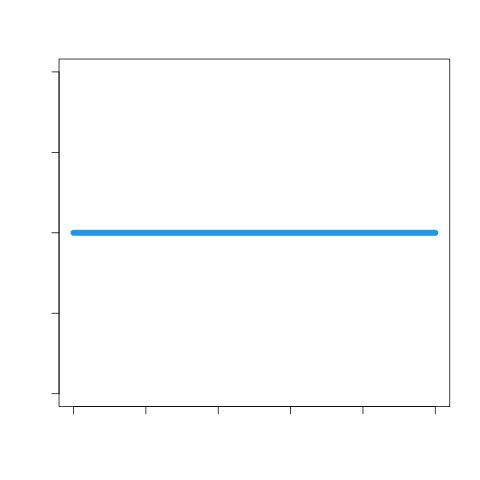
\includegraphics[width=.18\textwidth]{\fignet/FigMotifsBEDD-dist-g10} \end{tabular} &
    \begin{tabular}{c} 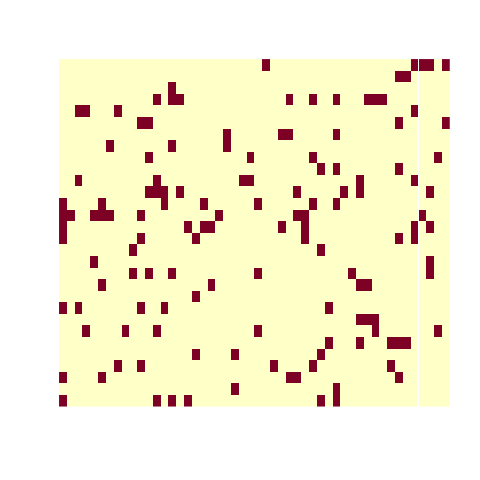
\includegraphics[width=.18\textwidth]{\fignet/FigMotifsBEDD-adj-g10-h10} \end{tabular} &
    \begin{tabular}{c} 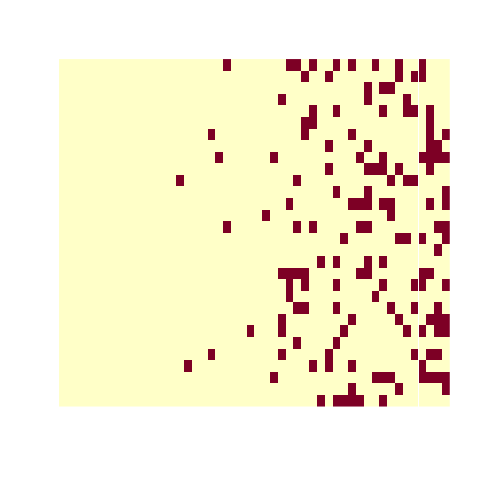
\includegraphics[width=.18\textwidth]{\fignet/FigMotifsBEDD-adj-g10-h40} \end{tabular} \\
    \begin{tabular}{r} $g =$ \end{tabular} &
    \begin{tabular}{c} 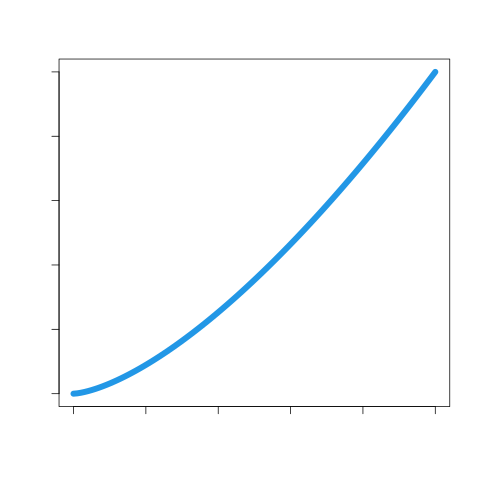
\includegraphics[width=.18\textwidth]{\fignet/FigMotifsBEDD-dist-g25} \end{tabular} &
    \begin{tabular}{c} 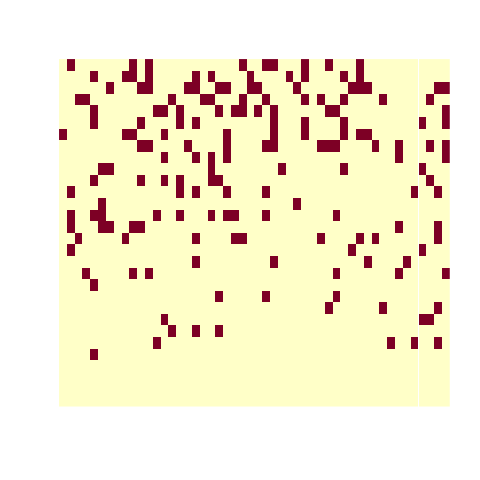
\includegraphics[width=.18\textwidth]{\fignet/FigMotifsBEDD-adj-g25-h10} \end{tabular} &
    \begin{tabular}{c} 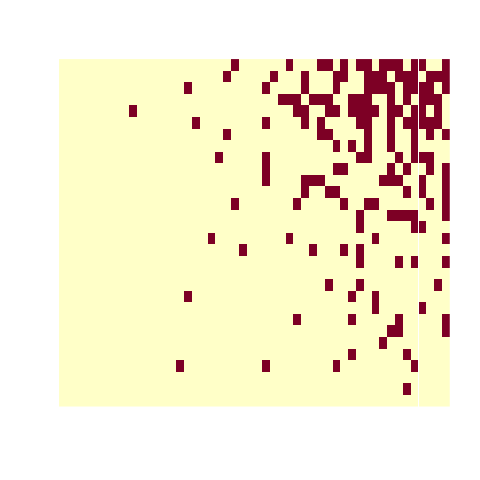
\includegraphics[width=.18\textwidth]{\fignet/FigMotifsBEDD-adj-g25-h40} \end{tabular} \\
  \end{tabular}
  
}

%====================================================================
\frame{\frametitle{Motif probability (1/2)} 

  \bigskip 
  \paragraph{\bEDD = row-column exhangeable,} so the motif probability
  $$
  \phi_s = \Pr(Y_s(\alpha) = 1)
  $$
  does not depend on the position $\alpha$.
  
  \bigskip \bigskip \bigskip \pause 
  \paragraph{Expected count.} Obviously
  $$
  \Esp(N_s) = c_s \phi_s, \qquad \Esp(F_s) = \phi_s.
  $$

  \bigskip \bigskip \pause
  \paragraph{Star motifs} (with degree $d$): under the \bEDD model,
  \begin{align*}
   \text{top star:} \qquad \emphase{\gamma_d} & : = \phibar_s = \rho^d \int g(u)^d \d u \comment{\left(\times \prod_{b=1}^q \int h(v_b) \d v_b\right)}\\
   \text{bottom star:} \qquad \emphase{\lambda_d} & := \phibar_s = \rho^d \int h(v)^d \d v
  \end{align*}
  Obviously $\rho = \gamma_1 = \lambda_1$.

}

%====================================================================
\frame{\frametitle{Motif probability (2/2)} 

  \bigskip
  \paragraph{General motif.} 
  \begin{align*}
    \Pbb\left(
    \includegraphics[width=.05\textwidth, trim=100 200 100 0]{\fignet/FigMotifsBEDD-motif9} 
    \right)
    & = 
    \frac{
    \overset{\text{top stars}}{\overbrace{
    \Pbb\left(\includegraphics[width=.05\textwidth, trim=100 200 100 0]{\fignet/FigMotifsBEDD-motif9-top1}\right) % \times 
    \Pbb\left(\includegraphics[width=.05\textwidth, trim=100 200 100 0]{\fignet/FigMotifsBEDD-motif9-top1}\right) % \times 
    \Pbb\left(\includegraphics[width=.05\textwidth, trim=100 200 100 0]{\fignet/FigMotifsBEDD-motif9-top2}\right)   }}
    \times
    \overset{\text{bottom stars}}{\overbrace{
    \Pbb\left(\includegraphics[width=.05\textwidth, trim=100 200 100 0]{\fignet/FigMotifsBEDD-motif9-bottom1}\right) % \times
    \Pbb\left(\includegraphics[width=.05\textwidth, trim=100 200 100 0]{\fignet/FigMotifsBEDD-motif9-bottom3}\right)
    }}
    }{
    \underset{\text{edges}}{\underbrace{
    \left(\Pbb\left(\includegraphics[width=.05\textwidth, trim=100 200 100 0]{\fignet/FigMotifsBEDD-motif9-top1}\right)\right)^4
    }}
    } \\
   \phibar_s & 
   = \frac{\gamma_1^2 \gamma_2 \lambda_1 \lambda_3}{\rho^4} 
   = \frac{\gamma_2 \lambda_3}{\rho} 
  \end{align*}

  \bigskip \pause
  \paragraph{That is} 
  $$
  \phibar_s = \left. \prod_{u = 1}^{p_s} \gamma_{d_u^s} \prod_{v = 1}^{q_s} \lambda_{e_v^s} \right/ \rho^{d_+^s}.
  $$
  where
  \begin{itemize}
   \item $d_u^s =$ degree of the $u$-th top node in motif $s$ (resp. $e_v^s$ for the $v$-th bottom node) \\ ~
   \item $d_+^s = \sum_u d_u^s = \sum_v e_v^s =$ number of edges in motif $s$
  \end{itemize}

}

%====================================================================
\frame{\frametitle{Variance of the count} 

  \hspace{-0.04\textwidth}
  \begin{tabular}{ll}
    \begin{tabular}{p{.5\textwidth}}
      \paragraph{Squared count:}
      $$
      \begin{array}{rcl}
        \Esp(N_s^2) & = & \Esp\displaystyle{\left(\sum_\alpha Y_s(\alpha)\right)^2} \\
        ~ \\
        & = & \displaystyle{\sum_{\alpha, \beta: \alpha \cap \beta = \emptyset} \Esp(Y_s(\alpha)) \; \Esp( Y_s(\beta))} \\
        ~ \\
        & & \displaystyle{+ \sum_{\alpha, \beta: \alpha \cap \beta \neq \emptyset} \underset{\footnotesize\begin{array}{c}\text{probability of} \\ \text{a 'super-motif'} \end{array}}{\underbrace{\Esp(Y_s(\alpha) Y_s(\beta))}}} \\
      \end{array}
      $$
      ~ \\ ~ \\
      \ra 'Close form' expression for the variance \\
      ~ \\ ~ \\ ~ \\ ~ \\ 
    \end{tabular} 
    &
    \begin{tabular}{p{.325\textwidth}}
      \paragraph{Motif:}
      $$
      \includegraphics[width=.075\textwidth, ]{\fignet/FigMotifsBEDD-motif9}
      $$
      \paragraph{Some super-motifs:} \\
      \includegraphics[width=.075\textwidth, ]{\fignet/FigMotifsBEDD-motif9-supermotif1} 
      \includegraphics[width=.075\textwidth, ]{\fignet/FigMotifsBEDD-motif9-supermotif2} 
      \includegraphics[width=.075\textwidth, ]{\fignet/FigMotifsBEDD-motif9-supermotif3} 
      \includegraphics[width=.075\textwidth, ]{\fignet/FigMotifsBEDD-motif9-supermotif4} \\
      \includegraphics[width=.075\textwidth, ]{\fignet/FigMotifsBEDD-motif9-supermotif5} 
      \includegraphics[width=.075\textwidth, ]{\fignet/FigMotifsBEDD-motif9-supermotif6} 
      \includegraphics[width=.075\textwidth, ]{\fignet/FigMotifsBEDD-motif9-supermotif7} 
      \includegraphics[width=.075\textwidth, ]{\fignet/FigMotifsBEDD-motif9-supermotif8} \\
      \includegraphics[width=.075\textwidth, ]{\fignet/FigMotifsBEDD-motif9-supermotif9} 
      \includegraphics[width=.075\textwidth, ]{\fignet/FigMotifsBEDD-motif9-supermotif10}
      \includegraphics[width=.075\textwidth, ]{\fignet/FigMotifsBEDD-motif9-supermotif11}
      \includegraphics[width=.075\textwidth, ]{\fignet/FigMotifsBEDD-motif9-supermotif12} \\
      \includegraphics[width=.075\textwidth, ]{\fignet/FigMotifsBEDD-motif9-supermotif13} 
      \includegraphics[width=.075\textwidth, ]{\fignet/FigMotifsBEDD-motif9-supermotif14}
      \includegraphics[width=.075\textwidth, ]{\fignet/FigMotifsBEDD-motif9-supermotif15}
      \includegraphics[width=.075\textwidth, ]{\fignet/FigMotifsBEDD-motif9-supermotif16} \\
      ~ \\
      \dots 396 super-motifs
    \end{tabular} 
  \end{tabular}
  
  \bigskip \pause
  \paragraph{Covariance:} same game, with $\Esp(Y_s(\alpha) Y_{s'}(\beta))$ for $s \neq s'$

}

%====================================================================
\frame{\frametitle{Plug-in estimates} 

  \paragraph{Motif probability estimate.} Denote by
  \begin{itemize}
   \item $\Gamma_d$ (resp. $\Lambda_d$) the frequency of the top (bottom) star with degree $d$,
   \item  $F_1$ the frequency of simple edges (graph density)
  \end{itemize}
  and define
  $$
  \Fbar_s = \left. \prod_{u = 1}^{p_s} \Gamma_{d_u^s} \prod_{v = 1}^{q_s} \Lambda_{e_v^s} \right/ F_1^{d_+^s}
  $$
  \ra Only depends on star counts 
  
  \bigskip \bigskip \bigskip \pause
  \paragraph{Moment estimates.}
  \begin{align*}
   \widehat{\Esp}(F_s) & = \Fbar_s, \\ ~ \\
   \widehat{\Var}(F_s) & = f(\Fbar_s, \Fbar_{\text{super-motifs}}), \\ ~ \\
   \widehat{\Cov}(F_s, F_{s'}) & = f(\Fbar_s, \Fbar_{s'}, \Fbar_{\text{super-motifs}}) \\
  \end{align*}

}

%====================================================================
\section{Asymptotic normality}
\frame{\frametitle{Outline} \tableofcontents[currentsection]}
%====================================================================
\frame{\frametitle{Asymptotic normality} 

  \paragraph{Asymptotic framework.} Consider a sequence of \bEDD graphs $\{G_N\}_{N \geq 1}$ with \\ ~
  \begin{itemize}
   \item dimension $m_N \times n_N$: $m_N = \lfloor \lambda N \rfloor$ (with $\lambda\in(0,1)$), $n_N = N -m_N$ \\ ~
   \item decreasing density $\rho_N = \Theta\left(m_N^{-a} n_N^{-b}\right)$ (with $a, b > 0$)  \\ ~
   \item constant functions $g$ and $h$
  \end{itemize}
  
  \bigskip \bigskip \bigskip \pause
  \paragraph{Main result.} For a motif $s$, such that $d_+^s < 2 / (a + b)$, 
  $$
  W_s := \frac{F_s - \Fbar_s}{\sqrt{\widehat{\Var}(F_s)}} \overset{D}{\longrightarrow} \Ncal(0, 1)
  $$

}

%====================================================================
\frame{\frametitle{Ingredients of the proof} 

  \paragraph{Martingale convergence.} ~ \\
  \begin{itemize}
  \item Use the conditional martingale $(F_s - \Esp(F_s \mid U, V))$ to prove that 
  $$
  \Var(F_s \mid U, V))^{-1/2}(F_s - \Esp(F_s \mid U, V)) \overset{D}{\rightarrow} \Ncal(0, 1)
  $$ \\ ~
  \item $\Var(F_s \mid U, V) / \Var(F_s) \rightarrow 1$ in probability.
  \end{itemize}


  \bigskip \bigskip \pause
  \paragraph{Control estimation errors.} 
  Under the sparsity condition $a + b < 2 / d_+^s$ \\ ~
  \begin{itemize}
   \item $\Var(F_s)^{-1/2} (\Fbar_s - \phibar_s) \rightarrow 0$ a.s.\\~ 
   \item $\widehat{\Var}(F_s) / {\Var}(F_s) \rightarrow 1$ in probability 
  \end{itemize}

  \bigskip \bigskip 
  \paragraph{Rk:} Some links with \refer{GaL17a}
}

%====================================================================
\frame{\frametitle{Corrected test statistic} 

  \paragraph{Claim.} Under \bEDD, for a given motif $s$, 
  $$
  W_s = (F_s - \Fbar_s) \left/ \; \sqrt{\widehat{\Var}(F_s)} \right. \approx \Ncal(0, 1)
  $$
  
  \bigskip \bigskip \pause
  \paragraph{Limitations of the plug-in estimates.} 
  $F_s$ and $\Fbar_s$ are not independent \\ ~ \\
  \ra For medium-size graphs, $\Var(F_s) \gg \Var(F_s - \Fbar_s)$ 
  
  \bigskip \bigskip \bigskip \pause
  \paragraph{Delta-method.} A second order Taylor expansion of 
  $$
  \Fbar_s(F_1, \{\Gamma_d\}, \{\Lambda_e\}) = \left. \prod_{u = 1}^{p_s} \Gamma_{d_u^s} \prod_{v = 1}^{q_s} \Lambda_{e_v^s} \right/ F_1^{d_+^s}
  $$
  provides estimates of $\mathbb{B}(\Fbar_s) = \Esp(\Fbar_s) - \phibar_s$ and $\Var(\Fbar_s)$ and, so, of $\Var(F_s - \Fbar_s)$ \\ ~ \\
  \ra Corrected statistic $\widetilde{W}_s = (\widehat{\Var}(F_s - \Fbar_s))^{-1/2}(F_s - \Fbar_s + \widehat{\mathbb{B}}(\Fbar_s))$.

}

%====================================================================
\section{Goodness-of-fit and network comparison}
\frame{\frametitle{Outline} \tableofcontents[currentsection]}
%====================================================================
\frame{\frametitle{Goodness-of-fit (1/2)} 

  \paragraph{Goodness-of-fit.} Reject $H_0 = \{G \sim \bEDD\}$ if
  $$
  W_s^2 = (F_s - \Fbar_s)^2 \left/ \; \widehat{\Var}(F_s) \right. > \chi^2_{1 - \alpha}
  $$

  \bigskip \pause
  \paragraph{qq-plots.} 
  $m = n = 2000$, $g(u) = 3 u^2$, $h(v) = 4 v^3$, $a = b = 1/3$ 
  
  $$
  \begin{tabular}{cccc}
%   motif 6 & motif 15 & motif 5 & motif 10 \\
  \includegraphics[width=.05\textwidth, trim=100 200 100 0]{\fignet/FigMotifsBEDD-motif6-automorphism1} &
  \includegraphics[width=.05\textwidth, trim=100 200 100 0]{\fignet/FigMotifsBEDD-motif15-automorphism1} &
  \includegraphics[width=.05\textwidth, trim=100 200 100 0]{\fignet/FigMotifsBEDD-motif5-automorphism1} &
  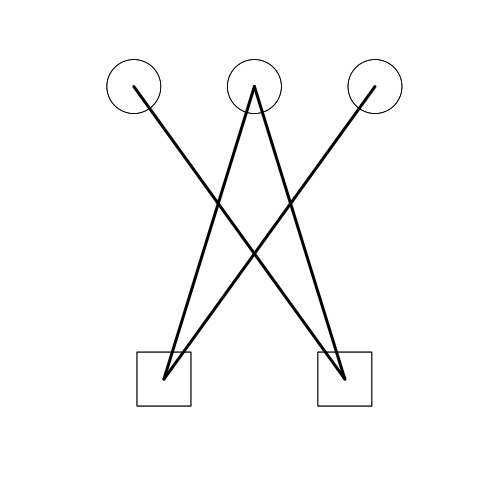
\includegraphics[width=.05\textwidth, trim=100 200 100 0]{\fignet/FigMotifsBEDD-motif10-automorphism1} \\
  \includegraphics[width=.2\textwidth, trim=10 10 10 10]{\fignet/AsymptoticNormality-mnRatio1-a33-b33-rhoCent1-g20-h30-S100-m2000-n2000-motif6} & 
  \includegraphics[width=.2\textwidth, trim=10 10 10 10]{\fignet/AsymptoticNormality-mnRatio1-a33-b33-rhoCent1-g20-h30-S100-m2000-n2000-motif15} &
  \includegraphics[width=.2\textwidth, trim=10 10 10 10]{\fignet/AsymptoticNormality-mnRatio1-a33-b33-rhoCent1-g20-h30-S100-m2000-n2000-motif5} & 
  \includegraphics[width=.2\textwidth, trim=10 10 10 10]{\fignet/AsymptoticNormality-mnRatio1-a33-b33-rhoCent1-g20-h30-S100-m2000-n2000-motif10}
  \end{tabular}
  $$
  
  $\bullet =$ raw statistic $W_s$, $\textcolor{blue}{\bullet} =$ \emphase{corrected statistic $\widetilde{W}_s$} \\~ \\
  $\textcolor{red}{-} = 95 \%$ CI for a qq-plot with 100 replicates
  
}

%====================================================================
\frame{\frametitle{Goodness-of-fit (2/2)} 

  \bigskip
  \paragraph{Corrected statistic.} $m = n \in \{10^1, \dots 10^3\}$, $\rho = 2.2 \; (mn) ^{-.4}$, all motifs
  $$
  \begin{array}{cccc}
  \Esp(N_s) < 1 & 1 \leq \Esp(N_s) < 10 &
  10 \leq \Esp(N_s) < 100  & \Esp(N_s) \geq 100 \\
  \includegraphics[width=.2\textwidth, trim=10 10 10 10]{\fignet/AsymptoticNormalityUnbiased-qqPlot-logExpCount0} & 
  \includegraphics[width=.2\textwidth, trim=10 10 10 10]{\fignet/AsymptoticNormalityUnbiased-qqPlot-logExpCount1} & 
  \includegraphics[width=.2\textwidth, trim=10 10 10 10]{\fignet/AsymptoticNormalityUnbiased-qqPlot-logExpCount2} & 
  \includegraphics[width=.2\textwidth, trim=10 10 10 10]{\fignet/AsymptoticNormalityUnbiased-qqPlot-logExpCount3} 
  \end{array}
  $$
  
  \bigskip \bigskip \pause
  \paragraph{Plant-pollinator networks.} $H_0$ almost always accepted ($10 < m, n < 10^3)$
  
  \bigskip \bigskip \pause \label{back:powerGOF}
  \paragraph{Power study.} ArXiv \refer{OLR21}: alternative = contamination with a stochastic block-model \\ ~ \\
  \ra Poor for $m = n \simeq 50$, ok for $m = n = 200$ 
  \Refer{\#\ref{goto:powerGOF}} 
}

%====================================================================
\frame{\frametitle{Network comparison} 

  \paragraph{Same degree imbalance for top nodes.} 
  \begin{itemize}
   \item Consider two networks $G^A \sim \bEDD(\rho^A, g^A, h^A)$ and $G^B \sim \bEDD(\rho^B, g^B, h^B)$, we want to test 
   $$
   H_0 = \{g^A = g^B\}
   $$ \\ ~ \pause
   \item Under $H_0$, $\gamma_d^A/(\rho^A)^d = \gamma_d^B/(\rho^B)^d$, so we may define 
   $$
   \widehat{\Esp}_0({\Gamma}_d^A) = \left(\frac{F_1^A}{F_1^B}\right)^d \Gamma_d^B
   \qquad \qquad (\text{idem for } \widehat{\Esp}_0({\Gamma}_d^B))
   $$
   to get estimates of  ${\Esp}_0(F_s^A)$, ${\Var}_0(F_s^A)$, ${\Esp}_0(F_s^B)$, ${\Var}_0(F_s^B)$, ... \\ ~ \\ ~ \pause
   \item Under $H_0$
   $$
   W_s = \frac{\left(F_s^A - \widehat{\Esp}_0(F_s^A)\right) - \left(F_s^B - \widehat{\Esp}_0(F_s^B)\right)}{\sqrt{\widehat{\Var}_0(F_s^A) + \widehat{\Var}_0(F_s^B)}}
   \overset{D}{\longrightarrow} \Ncal(0, 1)
   $$
  \end{itemize}

}

%====================================================================
\frame{\frametitle{Plant-pollinator vs Plant-seed disperser} 

  \paragraph{Data.} 
  \begin{itemize} 
  \item $G^A = 546 \times 1044$ plant-pollinator network
  \item $G^B = 207 \times 110$ plant-seed disperser network
  \end{itemize} 

  \bigskip \bigskip 
  \paragraph{Question.} Is there the same degree of imbalance between plants in the two networks ?

  \bigskip \bigskip 
  \paragraph{Results.} 
  $$
  \begin{array}{rccccc}
%   & \text{motif  5} & \text{motif 6} & \text{motif 10} & \text{motif 15} & \text{motif 16} \\
  &
  \includegraphics[width=.05\textwidth, trim=100 0 100 0, clip=]{\fignet/FigMotifsBEDD-motif5-automorphism1} &
  \includegraphics[width=.05\textwidth, trim=100 0 100 0, clip=]{\fignet/FigMotifsBEDD-motif6-automorphism1} &
  \includegraphics[width=.05\textwidth, trim=100 0 100 0, clip=]{\fignet/FigMotifsBEDD-motif10-automorphism1} &
  \includegraphics[width=.05\textwidth, trim=100 0 100 0, clip=]{\fignet/FigMotifsBEDD-motif15-automorphism1} &
  \includegraphics[width=.05\textwidth, trim=100 0 100 0, clip=]{\fignet/FigMotifsBEDD-motif16-automorphism1} \\ \hline ~ \\
  W_s: & -1.56 & -1.56 & -0.97 & -1.28 & -0.96 \\ ~ \\
  \widetilde{W}_s: & -2.71 & -1.90 & -1.76 & -1.34 & -0.96 \\
  \end{array}
  $$
  
  \bigskip \label{back:powerComp}
  \comment{Power study in \refer{OLR21}} \Refer{\#\ref{goto:powerComp}} 

}
%====================================================================
\section{Network embedding}
\frame{\frametitle{Outline} \tableofcontents[currentsection]}
%====================================================================
\frame{\frametitle{Network embedding} 

  \paragraph{Aim.} Analyse a set of $K$ networks $G^1, \dots G^K$
  
  \bigskip \bigskip 
  \paragraph{Principle.} Either
  \begin{itemize}
   \item[($a$)] summarize each network $G^k$ into a vector $x^k \in \Rbb^d$ or
   \item[($b$)]  compute a distance $d(k, k')$ between each pair of networks
  \end{itemize}
  then apply some multivariate analysis technique (principal component analysis, multi-dimensional scaling, clustering, ...)

  \bigskip \bigskip \pause
  \paragraph{Motif-based description.} Option ($a$), taking 
  \begin{align*}
   x_s^k & = N_s^k 
   & & \comment{\text{(sensitive to size, density, imbalance)}} \\ ~ \\
   x_s^k & = \left(N_s^k - \widetilde{\Esp}(N_s^k)\right) \left/ \sqrt{\widetilde{\Var}(N_s^k)}  \right.
   & & \comment{\text{(correction for size, density, imbalance)}} \\ ~ \\ 
   x_s & = \widetilde{\Var}(N^k)^{-1/2}\left(N^k - \widetilde{\Esp}(N^k)\right) 
   & & \comment{\text{(+ correction for correlation between counts)}}   
  \end{align*}

%   \begin{itemize}
%    \item $x_s^k = N_s^k$ \comment{(sensitive to size, density, imbalance)} \\ ~
%    \item $x_s^k = \widetilde{\Var}(N_s^k)^{-1/2}(N_s^k - \widetilde{\Esp}(N_s^k))$ \comment{(correction for size, density, imbalance)} \\ ~
%    \item $x_s = \widetilde{\Var}(N^k)^{-1/2}(N^k - \widetilde{\Esp}(N^k))$ \comment{(+ correction for for correlation between counts)}
%   \end{itemize}
  
}

%==================================================================
\frame{\frametitle{Zackenberg networks \refer{SRO16}}
  \bigskip
  \paragraph{Data.} $K = 46$ plant-pollinator networks, in two years, collected every few days

  \bigskip
  \begin{tabular}{c|c|c|c}
    \onslide+<1->{Raw counts PCA} & 
    \onslide+<2->{Bray-Curtis MDS} & 
    \onslide+<3->{Corr. stat. PCA} & 
    \onslide+<4>{Cholesky PCA} \\
    \hline
    \onslide+<1->{\includegraphics[width=.2\textwidth, height=.175\textheight]{\fignet/Zackenberg-red-PCAcount-scree}} &
    \onslide+<2->{\includegraphics[width=.2\textwidth, height=.175\textheight]{\fignet/Zackenberg-red-MDSBrayCurtis-scree}} & 
    \onslide+<3->{\includegraphics[width=.2\textwidth, height=.175\textheight]{\fignet/Zackenberg-red-PCAstat-scree}} &  
    \onslide+<4>{\includegraphics[width=.2\textwidth, height=.175\textheight]{\fignet/Zackenberg-red-PCAchol-scree}}
    \\
    \onslide+<1->{\includegraphics[width=.22\textwidth]{\fignet/Zackenberg-red-PCAcount-biplot}} &
    \onslide+<2->{\includegraphics[width=.22\textwidth]{\fignet/Zackenberg-red-MDSBrayCurtis-biplot}} &
    \onslide+<3->{\includegraphics[width=.22\textwidth]{\fignet/Zackenberg-red-PCAstat-biplot}} &
    \onslide+<4>{\includegraphics[width=.22\textwidth]{\fignet/Zackenberg-red-PCAchol-biplot}}
    \\
    \onslide+<1->{\includegraphics[width=.2\textwidth]{\fignet/Zackenberg-red-PCAcount-size}} &
    \onslide+<2->{\includegraphics[width=.2\textwidth]{\fignet/Zackenberg-red-MDSBrayCurtis-size}} &
    \onslide+<3->{\includegraphics[width=.2\textwidth]{\fignet/Zackenberg-red-PCAstat-size}} &
    \onslide+<4>{\includegraphics[width=.2\textwidth]{\fignet/Zackenberg-red-PCAchol-size}}
  \end{tabular}

}


%====================================================================
\section*{Discussion}
\frame{\frametitle{Outline} \tableofcontents[currentsection]}
%====================================================================
\frame{\frametitle{To conclude} 

  \paragraph{Summary.} 
  \begin{itemize}
   \item Motif counts provide a meso-scale desciption of a network \\~
   \item The bipartite EDD model accounts various typical network characteristics (density, degree imbalance) \\~
   \item Various test can be based on motif counts under \bEDD. Ex.:
   $$H_0 = \{G \sim \bEDD(g = 1)\}$$
   \ra Test for an absence of imbalance among the top nodes \comment{(no specialist vs generalist)}
  \end{itemize}
%   \begin{itemize}
%    \item $g \equiv 1$ implies that $\gamma_d = \rho^d$, so replace $\Gamma_d$ with $\widetilde{\Gamma}_d = (F_1)^d$ in all estimates: $\widetilde{F}_s, \widetilde{\Var}(F_s)$ \\~ 
%    \item reject $H_0$ if
%    $$
%    (F_s - \widetilde{F}_s)^2 \left/ \; \widetilde{\Var}(F_s) \right. > \chi^2_{1 - \alpha}
%    $$
%   \end{itemize}

  \bigskip \bigskip \bigskip \pause
  \paragraph{Extensions \& alternative leads.} 
  \begin{itemize}
   \item Which alternatives are best captured by each motif? \\ ~ 
   \item Understanding species roles in networks \\ ~ 
   \item $U$-statistics in row-column exchangeable models \refer{LeM21}
  \end{itemize}

}

%====================================================================
\frame[allowframebreaks]{ \frametitle{References}
  {
   \tiny
   \bibliography{/home/robin/Biblio/BibGene}
   \bibliographystyle{alpha}
  }
}

%====================================================================
\backupbegin
\section*{Appendix}
%====================================================================
\frame{\frametitle{Power study: goodness-of-fit} 

  \paragraph{Alternative:} 2-block stochastic block model \label{goto:powerGOF}
  $$
  \includegraphics[width=.8\textwidth]{\fignet/OLR21-ArXiv-Fig5}
  $$
  \Refer{\#\ref{back:powerGOF}} 

}

%====================================================================
\frame{\frametitle{Power study: network comparison} 

  \paragraph{Alternative:} 2-block stochastic block model \label{goto:powerComp}
  $$
  \includegraphics[width=.8\textwidth]{\fignet/OLR21-ArXiv-Fig6}
  $$
  \Refer{\#\ref{back:powerComp}} 
}

%====================================================================
\backupend
%====================================================================

%====================================================================
%====================================================================
\end{document}
%====================================================================
%====================================================================
  
  \hspace{-.025\textwidth}
  \begin{tabular}{cc}
    \begin{tabular}{p{.5\textwidth}}
    \end{tabular}
    & 
    \hspace{-.02\textwidth}
    \begin{tabular}{p{.5\textwidth}}
    \end{tabular}
  \end{tabular}

